%\documentclass[a4paper, twoside] {thesis}
%\usepackage{amsmath}
%\usepackage{esvect}
%\usepackage{amssymb}
%\usepackage{cclicenses}
%\usepackage{graphicx}
%\begin{document}
\chapter{Chapter 2}
\section{Theoretical work}

\subsection{EMW Equation In Vacuum}
Electromagnetic wave equation is one of the consequences of Maxwell’s equations.\\
As in vacuum charge density $\rho$ and current density J vanishes, So Maxwell's equations becomes:\\
1. Gauss’s Law For Electricity\\
\begin{equation}
\vec{\nabla}.\vec{E} = 0
\end{equation}
2. Gauss’s Law For Magnetism\\
\begin{equation}
\vec{\nabla}.\vec{B} = 0
\end{equation}
3. Faraday’s Law Of Induction\\
\begin{equation}
\vec{\nabla}\times\vec{E} = - \frac{\partial\vec{B}}{\partial t}
\end{equation}
4. Ampere’s Law\\
\begin{equation}
\vec{\nabla}\times\vec{B} = \mu_{o}\epsilon_{o}\frac{\partial\vec{E}}{\partial t}
\end{equation}
Now if we apply curl to Eq. 1.3\\
\begin{equation}
\vec{\nabla}\times(\vec{\nabla}\times\vec{E}) = - \vec{\nabla}\times(\frac{\partial\vec{B}}{\partial t})
\end{equation}
using the definition of second derivative;\\
\begin{equation}
\vec{\nabla}\times(\vec{\nabla}\times\vec{A}) = \vec{\nabla}(\vec{\nabla}.\vec{A})-{\nabla}^2A
\end{equation}
Eq. 1.5 becomes\\
\begin{equation}
\vec{\nabla}(\vec{\nabla}.\vec{E})-{\nabla}^2E = - \frac{\partial}{\partial t}(\vec{\nabla}\times\vec{B})
\end{equation}
from Eqs. 1.1 and 1.4\\
\begin{equation}
\nabla^2\vec{E} =  \mu_{o}\epsilon_{o}\frac{\partial^2\vec{E}}{\partial t^2}
\end{equation}
Here each component of $\vec{E}$ satisfies the EMW equation for electric field.\\ 
Similarly by applying curl to Eq. 1.4, we get the EMW equation for magnetic field.\\
i.e,\\
\begin{equation}
\nabla^2\vec{B} =  \mu_{o}\epsilon_{o}\frac{\partial^2\vec{B}}{\partial t^2}
\end{equation}
where \\
$\mu_{o} = 1.257\times10^{-6} mkgs^{-2}A^{-2}$\\
$\epsilon_{o} = 8.854\times10^{-12} m^{-3}kg^{-1}s^4A^2$\\
So\\
\begin{equation}
\frac{1}{\sqrt{\mu_{o}\epsilon_{o}}} = 3\times10^8 ms^{-1}
\end{equation}
which is equal to speed of light, c.\\
This means that EMW can travel through vacuum with the speed equals to speed of light, So light is an EMW, where elctric field $\vec{E}$ and magnetic field $\vec{B}$ are perpendicular to each other and also to the direction of propagation of light/EMW.

\subsection{Poynting Vector}
The Poynting vector $\vec{S}$ represents the directional energy flux i.e, the energy transfer per unit area per unit time of an electromagnetic field.\\
\begin{equation}
\vec{S} = \frac{1}{\mu_{o}}(\vec{E}\times\vec{B})
\end{equation}
Which shows that the direction of power flow (propagation of EMW) at any point is normal to both $\vec{E}$ and $\vec{B}$.\\
This implies that EMW/light is an Transverse wave.\\
The SI unit of the Poynting vector is the watt per square meter, $W/m^{-2}$.

\subsection{Wave Solution In Spherical Coordinates}

\subsubsection{Spherical Coordinate System}
Vector derivatives in spherical coordinates are as:\\
Gradient\\
\begin{equation}
\vec{\nabla} A = \frac{\partial A}{\partial r}\hat{r}+\frac{1}{r}\frac{\partial A}{\partial \theta}\hat{\theta}+\frac{1}{r\sin\theta}\frac{\partial A}{\partial \phi}\hat{\phi}
\end{equation}
Divergence\\
\begin{equation}
\vec{\nabla}.\vec{A} = \frac{1}{r^2}\frac{\partial}{\partial r}(r^2A_r)+\frac{1}{r\sin\theta}\frac{\partial}{\partial\theta}(\sin\theta A_\theta)+\frac{1}{r\sin\theta}\frac{\partial A_\phi}{\partial\phi}
\end{equation}
Curl\\
\begin{equation}
\vec{\nabla}\times\vec{A} = \frac{1}{r\sin\theta}[\frac{\partial}{\partial\theta}(\sin\theta A_\phi)-\frac{\partial A_\theta}{\partial\phi}]\hat{r}+\frac{1}{r}[\frac{1}{\sin\theta}\frac{\partial A_r}{\partial\phi}-\frac{\partial}{\partial r}(rA_\phi)]\hat{\theta}+\frac{1}{r}[\frac{\partial}{\partial r}(rA_\theta)-\frac{\partial A_r}{\partial \theta}]\hat{\phi}
\end{equation}
Laplacian\\
\begin{equation}
\nabla^2 \vec{A} = \frac{1}{r^2}\frac{\partial}{\partial r}(r^2\frac{\partial\vec{A}}{\partial r})+\frac{1}{r^2\sin\theta}\frac{\partial}{\partial\theta}(\sin\theta\frac{\partial\vec{A}}{\partial \theta})+\frac{1}{r^2\sin^2\theta}\frac{\partial^2\vec{A}}{\partial \phi^2}
\end{equation}

\subsubsection{Wave Solution}
Starting from wave equation,\\
\begin{equation}
\vec{\nabla}^2\vec{E}(\vec{s},t) =  \frac{1}{c^2}\frac{\partial^2\vec{E}(\vec{s},t)}{\partial t^2}
\end{equation}
where\\
$\vec{E}(\vec{s},t) = \vec{E}(\vec{r},\vec{\theta},\vec{\phi},t)$
and using laplacian from Eq. 1.15;\\
Eq. 1.16 becomes\\
\begin{equation}
\frac{1}{r^2}\frac{\partial}{\partial r}(r^2\frac{\partial\vec{E}(\vec{r},\vec{\theta},\vec{\phi},t) }{\partial r})+\frac{1}{r^2\sin\theta}\frac{\partial}{\partial\theta}(\sin\theta\frac{\partial \vec{E}(\vec{r},\vec{\theta},\vec{\phi},t)}{\partial \theta})+\frac{1}{r^2\sin^2\theta}\frac{\partial^2\vec{E}(\vec{r},\vec{\theta},\vec{\phi},t)}{\partial \phi^2} = \frac{1}{c^2}\frac{\partial^2\vec{E}(\vec{r},\vec{\theta},\vec{\phi},t)}{\partial t^2}
\end{equation}
For spherical symmetry, motion is radial which means $\theta$ and $\phi$ are constants,\\
\begin{equation}
\frac{1}{r^2}\frac{\partial}{\partial r}(r^2\frac{\partial\vec{E}(\vec{r},t) }{\partial r})+\frac{1}{r^2\sin\theta}\frac{\partial}{\partial\theta}(\sin\theta\frac{\partial \vec{E}(\vec{r},t)}{\partial \theta})+\frac{1}{r^2\sin^2\theta}\frac{\partial^2\vec{E}(\vec{r},t)}{\partial \phi^2} = \frac{1}{c^2}\frac{\partial^2\vec{E}(\vec{r},t)}{\partial t^2}
\end{equation}
where\\

$\frac{\partial^2\vec{E}(\vec{r},t)}{\partial \theta^2}$ and $\frac{\partial^2\vec{E}(\vec{r},t)}{\partial \phi^2}$ become zero and we are left with;\\
\begin{equation}
\frac{1}{r^2}\frac{\partial}{\partial r}(r^2\frac{\partial\vec{E}(\vec{r},t) }{\partial r}) = \frac{1}{c^2}\frac{\partial^2\vec{E}(\vec{r},t)}{\partial t^2}
\end{equation}
\begin{equation}
\frac{1}{r^2}[r^2\frac{\partial^2\vec{E}(\vec{r},t)}{\partial r^2}+\frac{\partial\vec{E}(\vec{r},t) }{\partial r}.(2r)] = \frac{1}{c^2}\frac{\partial^2\vec{E}(\vec{r},t)}{\partial t^2}
\end{equation}
By solving left hand side of the Eq. 1.20, we get;\\
 $\frac{1}{r}\frac{\partial^2}{\partial r^2}[r\vec{E}(\vec{r},t)]$\\
So, Eq. 1.20 becomes;\\
\begin{equation}
\frac{1}{r}\frac{\partial^2}{\partial r^2}[r\vec{E}(\vec{r},t)] = \frac{1}{c^2}\frac{\partial^2\vec{E}(\vec{r},t)}{\partial t^2} 
\end{equation}
Multiplying by r\\
\begin{equation}
\frac{\partial^2}{\partial r^2}[r\vec{E}(\vec{r},t)] = \frac{r}{c^2}\frac{\partial^2\vec{E}(\vec{r},t)}{\partial t^2} 
\end{equation}
Writing it as;\\
\begin{equation}
\frac{\partial^2}{\partial r^2}[r\vec{E}(\vec{r},t)] = \frac{1}{c^2}\frac{\partial^2}{\partial t^2}[r\vec{E}(\vec{r},t)]
\end{equation}
Let $r\vec{E}(\vec{r},t) = \vec{T}(\vec{r},t)$\\
Now, Eq. 1.23 becomes;\\
\begin{equation}
\frac{\partial^2}{\partial r^2}[\vec{T}(\vec{r},t)] = \frac{1}{c^2}\frac{\partial^2}{\partial t^2}[\vec{T}(\vec{r},t)]
\end{equation}
This is a wave equation in one dimension, with solution;\\
\begin{equation}
\vec{T}(\vec{r},t) = \exp{i(kr-wt)}\hat{r}
\end{equation}
Or it can be written as;\\
\begin{equation}
\vec{T}(\vec{r},t) = \sin(kr-wt)
\end{equation}
As $r\vec{E}(\vec{r},t) = \vec{T}(\vec{r},t)$\\
So;\\
\begin{equation}
r\vec{E}(\vec{r},t) = \sin(kr-wt)
\end{equation}
And the final solution of wave equation is;\\
\begin{equation}
\vec{E}(\vec{r},t) = \frac{1}{r}\sin(kr-wt)
\end{equation}

\subsection{Charge Density}
Charge density $\rho$ is a measure of electric charge per unit volume of space, in one, two or three dimensions.\\
More specifically, We have;\\
1. Linear charge density: is the amount of electric charge per unit length.\\
2. Surface charge density: is the amount of electric charge per surface area.\\
3. Volume charge density: is the amount of electric charge per volume.\\
From Gauss's law for electricity;\\
\begin{equation}
\vec{\nabla}.\vec{E} = \frac{\rho}{\epsilon_{o}}
\end{equation}
Charge density $\rho$ is\\
\begin{equation}
\rho = {\epsilon_{o}}(\vec{\nabla}.\vec{E})
\end{equation}
Now by using the equation for divergence, Eq. 1.13 and for $\vec{E}$, Eq. 1.28;\\
\begin{equation}
\rho = {\epsilon_{o}}[\frac{1}{r^2}\frac{\partial}{\partial r}(r^2\frac{1}{r}\sin(kr-wt))]
\end{equation}
\begin{equation}
\rho = {\epsilon_{o}}[\frac{1}{r^2}\frac{\partial}{\partial r}(r\sin(kr-wt))]
\end{equation}
\begin{equation}
\rho = {\epsilon_{o}}[\frac{1}{r^2}(r\cos(kr-wt).k+\sin(kr-wt))]
\end{equation}
Final equation for charge density is;\\
\begin{equation}
\rho = {\epsilon_{o}}[\frac{k}{r}\cos(kr-wt)+\frac{1}{r^2}\sin(kr-wt)]
\end{equation}
Which is not equal to zero, but it should be as we considered the case for vacuum; where there are no any charges and no charge density accordingly.\\

\subsection{Problem}
As determined solution Eq. 1.28, for wave equation in vacuum Eq. 1.16, is mathematically true and have no issue, But;\\
Why we did not get zero charge density?

\subsection{Solution}
The wave solution;\\
\begin{equation}
\vec{E}(\vec{r},t) = \frac{1}{r}\sin(kr-wt)
\end{equation}
is invalid for EMWs but is valid for acoustic/sound waves.\\

\subsubsection{Reason}
From Eq. 1.11, EMWs are transverse waves, but sound waves are longitudinal waves.\\
As we had spherically symmetric EMWs over a central point;
Carrying equal energy in all directions means isotropic EMWs.\\
And if we consider a sphere about the central point, at a large radius, then at that radius the wave over a reasonable area is essentially planar. We know electric and magnetic field of a plane wave in free space is always perpendicular to the direction of propagation of wave.\\
So, The electric field would have to be tangent to the surface of sphere everywhere, and continuous along that surface; Which means we have a continuous vector field, tangent to the surface of a sphere.\\
Now???\\
According to Hairy Ball Theorem
\begin{center}
	"For a sphere, If f is a continuous function that assigns a vector in $R^3$ to every point p on the sphere such that f(p) is always tangent to the sphere at point p then there is at least one point p such that f(p)=0."\\
\end{center}
This means that a continuous vector field, tangent to the surface of a sphere must fall to zero at one or more points on the sphere.\\
Which is inconsistent with the assumption of an isotropic EMWs.

\subsection{Isotropic Antenna}
As spherically isotropic EMWs are not possible, so there are no real isotropic radiators for EMWs, and because of this an isotropic electromagnetic antenna is a hypothetical antenna which does not exist in actual.\\
But, isotropic sound waves are possible as they are longitudinal waves and does not have any perpendicular component.

\section{Computational Work}
Our task is to construct the plot between distance and intensity, for multiple antenna sources arrange in a linear array and by managing phase between them we get a directive beam with maximum intensity .\\
First, we have to figure out an equation for intensity.\\
Let, we have a single source which is at distance L from the point of observation x=0, Now find the intensity at any point, say x from x=0, which is at distance r from the source?\\
As intensity is defined as power transferred per unit area, where the area is measured on the plane perpendicular to the direction of propagation of the energy. which is same as poynting vector, So by using the Eq. 1.11 for finding intensity.\\
\begin{equation}
I = \frac{1}{\mu_{o}}(\vec{E}\times\vec{B})
\end{equation}
Where $\vec{B} = \vec{E}/c$,\\
\begin{equation}
I = \frac{\sqrt{\mu_{o}{\epsilon_{o}}}}{\mu_{o}}E^2
\end{equation}
\begin{equation}
I = c\epsilon_{o}E^2
\end{equation}
So,\\
Intensity is directly proportional to square of electric field, i.e\\
\begin{equation}
I \propto E^2
\end{equation}
From Eq. 1.28, electric field for point at origin is ,\\
\begin{equation}
\vec{E}(\vec{r},t) = \frac{1}{r}\sin(kr-wt)\hat{r}
\end{equation}
And for the point x from x=0, at distance r from the source;\\
$r(x) = \sqrt{L^2+x^2}$ and $\hat{r} = \cos\theta\hat{x}+\sin\theta\hat{y}$\\
So,\\
Electric field component along x-axis is\\
\begin{equation}
\vec{E}_x(x,t) = \frac{x}{r^2}\sin(kr-wt)
\end{equation}
and;\\
Electric field component along y-axis is\\
\begin{equation}
\vec{E}_y(x,t) = \frac{L}{r^2}\sin(kr-wt)
\end{equation}
Final equation for intensity becomes;\\
\begin{equation}
I = E_x^2(x,t)+E_y^2(x,t)
\end{equation}
Now, by using python, plot distance and intensity for the single source;\\
\begin{verbatim}
import matplotlib.pyplot as plt
from math import sqrt, sin
w=1 #(t'=wt)
k=1 #(r'=kr)
L=1

def r(x):
return sqrt(L**2+x**2)

def Ex(x,t):
return (x/r(x)**2)*(sin(k*r(x)-w*t))

def Ey(x,t):
return (L/r(x)**2)*(sin(k*r(x)-w*t))

print(Ex(3,1))
print(Ey(3,1))

def I(x,t):
return (Ex(x,t)**2+Ey(x,t)**2)

print(I(3,5))

#plot between intensity and distance.
a=[]
b=[]
for i in range(-150,150,1):
x=i/10.0
y=I(x,0)
a.append(x)
b.append(y)
#x= x+1
fig= plt.figure()
axes=fig.add_subplot(111)
axes.plot(a,b)
plt.show()
\end{verbatim}

\begin{figure}[ht]
\centering	
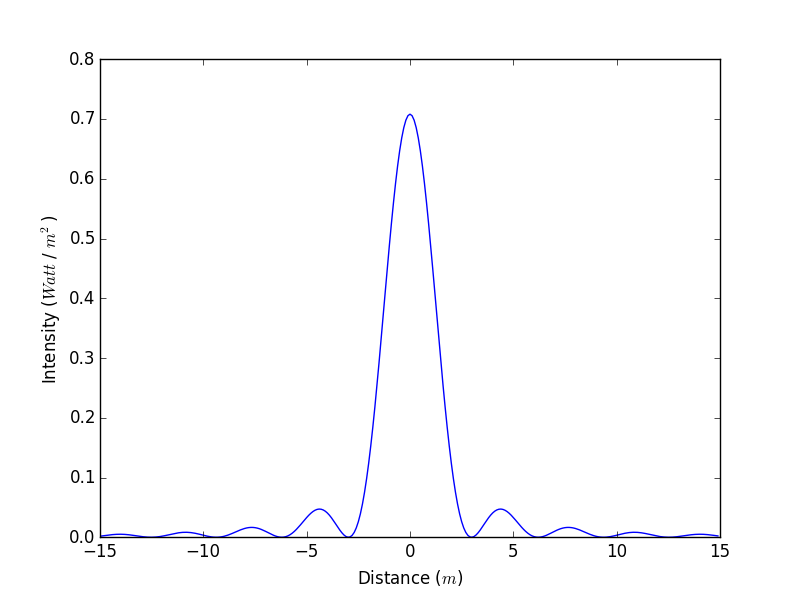
\includegraphics[scale=0.45]{figure_1.png}
\caption{Plot between distance and intensity}
\end{figure}

\begin{flushleft}
	As it should be, Intensity decreases by increasing the distance. Where at the position where source is placed we have high intensity peak.
\end{flushleft}
Next;\\
Plot between distance and intensity, for four antenna sources arrange in a linear array and by managing phase between them, we get interference pattern.
\begin{verbatim}
import numpy as np
import matplotlib.pyplot as plt
from math import sqrt, sin, pi

w=1.0
k=1.0
L=10.0 / k
P=0
# Calculate fringe spacing:
#d = 2 * 5           # Slit-spacing
#fs = 2 * pi * L / (k * d)

#print("Slit-spacing = {} produces fringe spacing = {}".format(d, fs))

ds = [-12, -4, 4, 12]
#sources=[(distance,phase)]
sources = [(-12, 0), (-4,0), (4,0), (12,0)]

def r(x,d):
return sqrt(L**2+(x-d)**2)

def Ex(x,d,p,t):
return ((x-d)/r(x,d)**2)*(sin(k*r(x,d)-w*t+p))

def Ey(x,d,p,t):
return (L/r(x,d)**2)*(sin(k*r(x,d)-w*t+p))

def I(x,sources,t):
Ox=0
Oy=0
for d, p in sources:
Ox+=Ex(x,d,p,t)
Oy+=Ey(x,d,p,t)

return Ox**2+Oy**2

def trapezoidal(f, a, b, n):
h = float(b - a) / n
s = 0.0
s += f(a)/2.0
for i in range(1, n):
s += f(a + i*h)
s += f(b)/2.0
return s * h

xs=[]
ys=[]

for x in np.linspace(-20,20,1000):
y = trapezoidal(lambda t: I(x,sources,t), -pi/w, pi/w, 100) / (2 * pi)

xs.append(x)
ys.append(y)

plt.plot(xs,ys)
plt.show()   
\end{verbatim}
\begin{figure}[ht]
	\centering	
    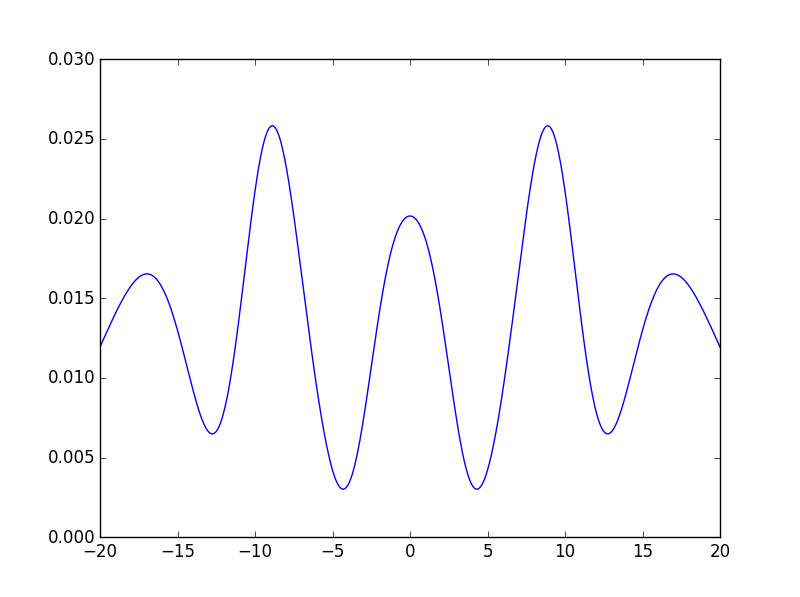
\includegraphics[scale=0.45]{figure_2.png}
	\caption{Plot between distance and intensity}
\end{figure}



%\end{document}
